\section{Die Fraunhofer Gesellschaft}
%------------------------------------------------------------------------
\mode<presentation>{
  \begin{frame}[t] \frametitle{Forschungsprofil der Fraunhofer Gesellschaft}
    \begin{itemize}
    \item gr\"o\ss te Forschungseinrichtung f\"ur anwendungsorientierte Forschung in Europa 
      \begin{itemize}
      \item[Ziel]: ergebnisorientierte Forschung zum unmittelbaren Nutzen f\"ur die Wirtschaft und zum Vorteil der Gesellschaft
      \end{itemize}
    \end{itemize}

    \begin{itemize}
    \item mehrere Forschungsthemen, u.a. 
      \begin{itemize}
      \item Energie und Wohnen
      \item Verkehr und Mobilit\"at
      \item ...
      \end{itemize}
    \end{itemize}

    \begin{columns}
      \begin{column}{0.5\textwidth}
        \begin{itemize}
        \item Gleichgewicht zwischen anwendungsorientierter Grundlagenforschung und innovativer Entwicklung
        \item Finanzierung \"uber Auftragsforschung (70\%) und \"offentliche Gelder (30\%) 
        \end{itemize}
      \end{column}
      \begin{column}{0.45\textwidth}
        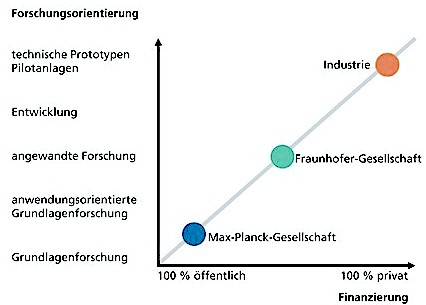
\includegraphics[width=1\textwidth]{pics/finanzenFraunhofer}
      \end{column}
    \end{columns}
  \end{frame}
}

%------------------------------------------------------------------------
\begin{frame}[t] \frametitle{Struktur der Fraunhofer Gesellschaft}
  \begin{columns}
    \onslide<1-2>{
    \begin{column}{0.55\textwidth}
      \begin{itemize}
      \item etwa 22.000 Mitarbeiter, \"uberwiegend Naturwissenschaftler und Ingenieure
      \item dezentrale Organisation durch 
        \begin{itemize}
        \item 66 Fraunhofer-Institute
        \item 10-20 kleinere Forschungseinrichtungen
        \item weitere Niederlassungen au\ss erhalb Deutschlands
        \end{itemize}
      \item Zentrale in M\"unchen
      \item 40 Standorte in Deutschland, darunter auch z.B. SCAI in Sankt-Augustin
      \item die Institute sind in ``Verb\"unden'' zusammengefasst
      \end{itemize}
    \end{column}}
    \begin{column}{0.40\textwidth}
      \invisible<1>{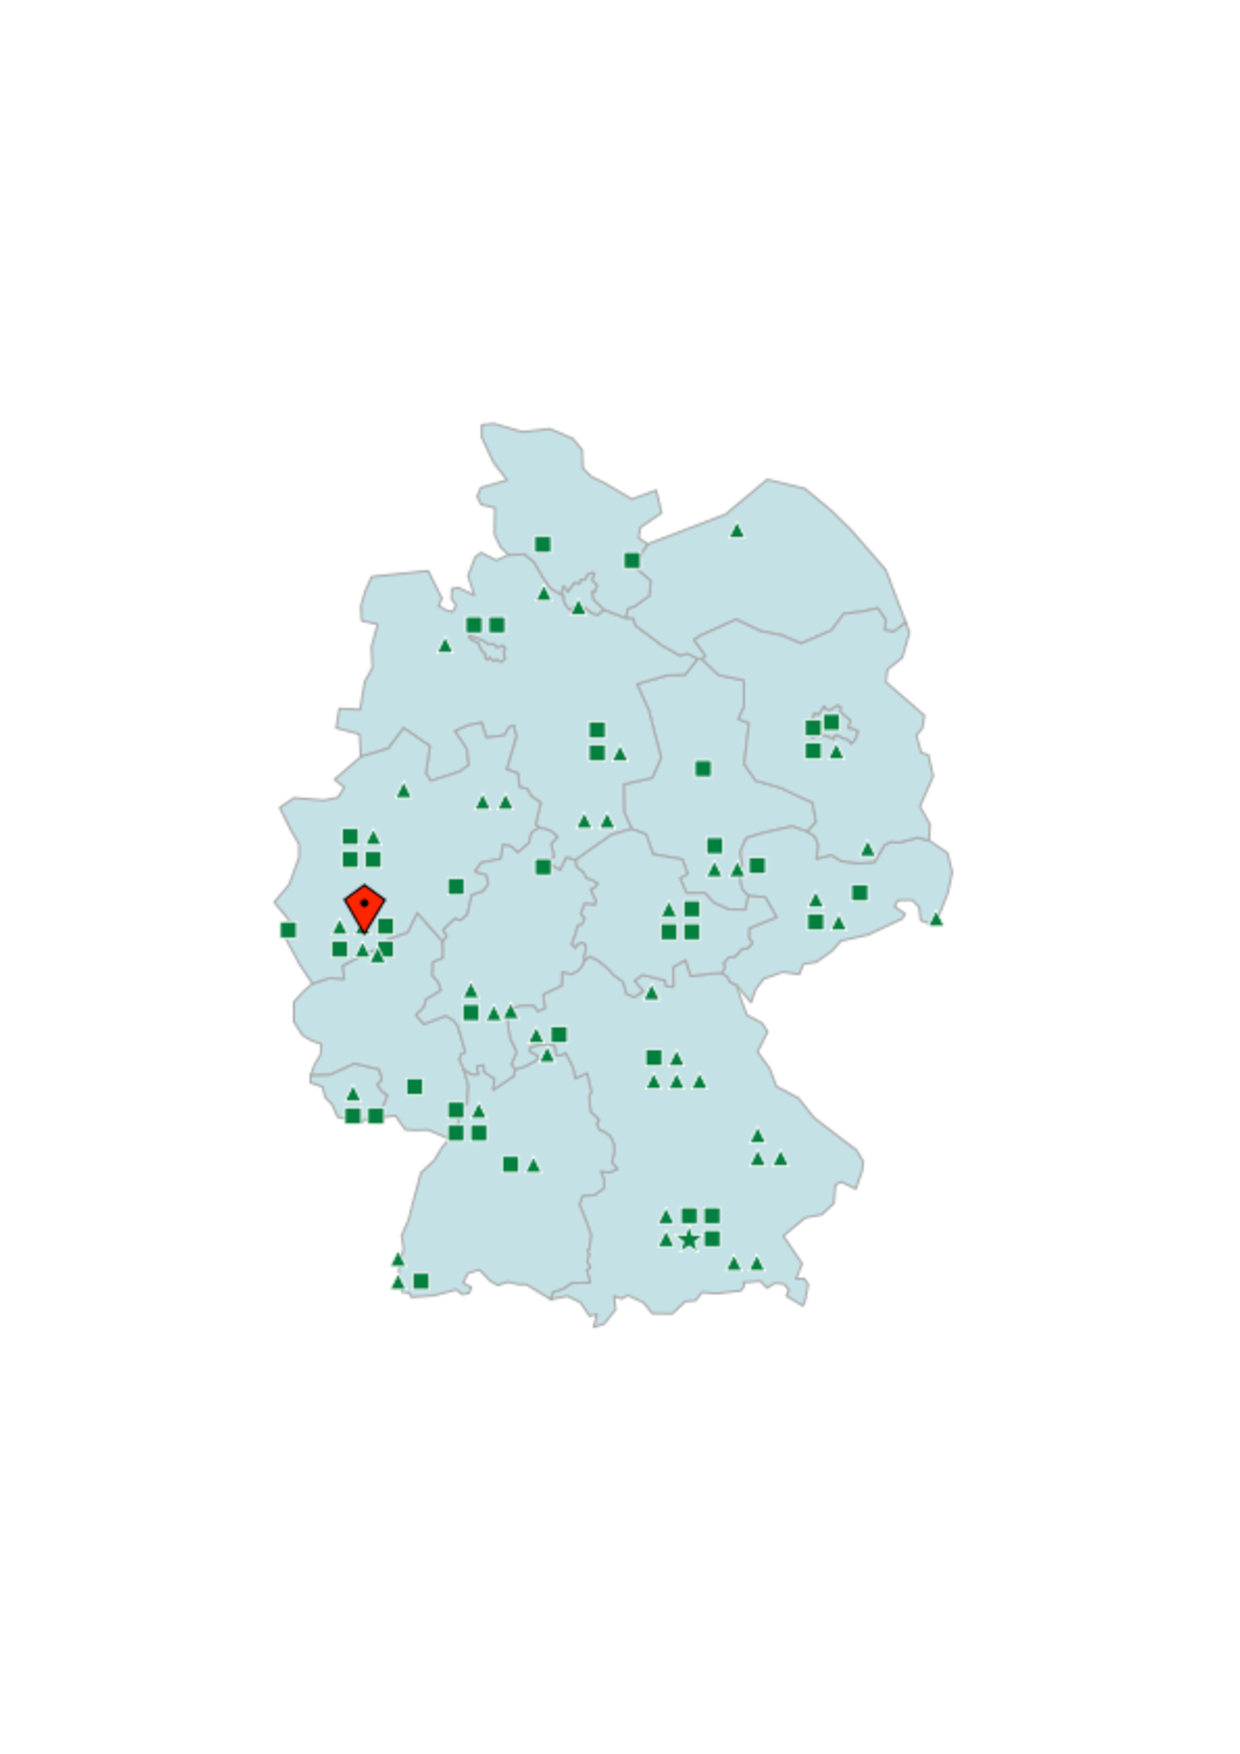
\includegraphics[width=1.0\textwidth]{pics/mapFraunhofer}}
    \end{column}
  \end{columns}
\end{frame}

%------------------------------------------------------------------------

